\subsection{Antagonism}\label{antagonism}

A fundamental principle in the body plan of bilaterians is the organization of movement through antagonistic pairs of effectors. Muscles, by their biological constitution, can only contract (i.e., pull) but not push. This morphological constraint necessitates the evolution of opposing pairs of muscles—flexors and extensors, abductors and adductors, pronators and supinators—that can act in reciprocal fashion to enable controlled motion \cite{Huxley1932_RelativeGrowth,Schilling2011_AntagonisticEvolution}. The bilaterian body plan, with its segmentation and bilateral symmetry, provides the structural basis for this arrangement.

At the neural level, antagonism is implemented by the canonical circuit motif of reciprocal inhibition. Sherrington’s classic work established that the activation of one muscle in a pair is accompanied by inhibition of its antagonist, ensuring coordinated and efficient movement \cite{Sherrington1906_IntegrativeAction}. This basic inhibitory scheme remains central to vertebrate and invertebrate motor control and underlies the formation of stable motor patterns.

From a biomechanical perspective, antagonistic control confers several advantages. Co-activation of antagonists allows modulation of joint stiffness, enabling both stability and compliance. Such mechanisms are critical for adaptive interaction with the environment and have inspired numerous robotic implementations of antagonistic actuators \cite{Hogan1984_ImpedanceControl,Tondu2012_McKibbenMuscle}. In biological systems, this provides the capacity not only to move but also to regulate impedance and precision.

In the context of the sensation-modulating network (SMN), antagonism is not merely a mechanical solution but also a higher-order organizational principle. Antagonistic structures encode dynamic balances: approach versus avoidance, activation versus inhibition, flexion versus extension. These embodied oppositions structure the repertoire of available action schemas and affordances, contributing to the cognitive architecture of the SMN itself \cite{Bizzi2013_MuscleSynergies}. Thus, antagonism serves as both a morphological constraint and a generative principle for embodied cognition.

\begin{figure}[htbp]
  \centering
  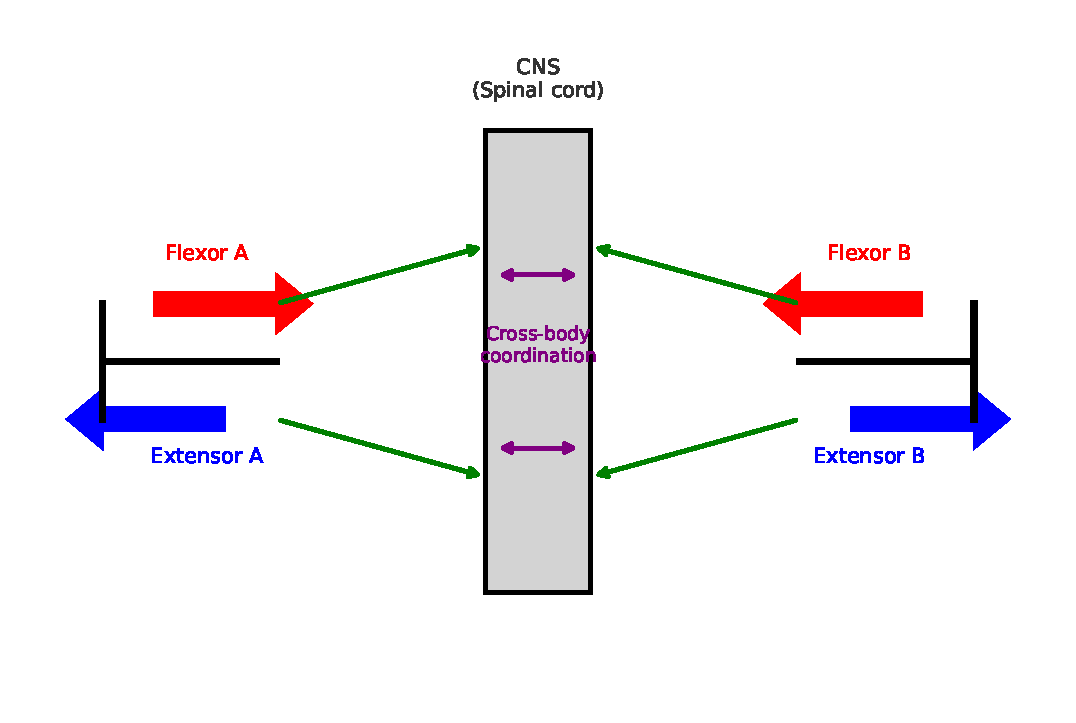
\includegraphics[width=0.8\textwidth]{graphics/smn_antagonism_bilateral_cns.pdf}
  \caption{%
    Antagonism at multiple levels of the body plan. 
    Local antagonism operates between flexor and extensor pairs within each action zone (red and blue arrows). 
    Reciprocal inhibition is mediated through central nervous system pathways (green arrows into the spinal cord). 
    Cross-body coordination (purple arrows) connects bilaterally symmetrical zones, showing how antagonism is both a morphological and neural principle.%
  }
  \label{fig:smn-antagonism}
\end{figure}

\subsubsection{Antagonistic Architecture could Generate Fixed and Haltable Action Patterns}
Antagonism as an explanatory theme in biology is widely recognized. The role of agonistic and antagonistic muscles in motor coordination is well established. Each action zone may have multiple sets of agonist and antagonist \textit{actors}.  A contraction leading to a pull of agonist alternated by an antagonist's pull may generate a simple open-close pattern, one cycle: one fixed action pattern (FAP). 

This can be modeled as a Petri net \cite{peterson1977petri}, a bipartite graphical representation used widely for modeling processes as changing states are affected by transitions. The two kinds of nodes in the graph are places and transitions. A transition has a prior state represented as an input place value (token) and a post-state as a resulting place value. 

For example, a sense organ as a transducer can be represented as a transition of an analog physical perturbation from the environment (an input) into an action potential within the agent. This transduction is the basic source of input tokens to the agent, forming sensations.
\begin{figure}[ht] 
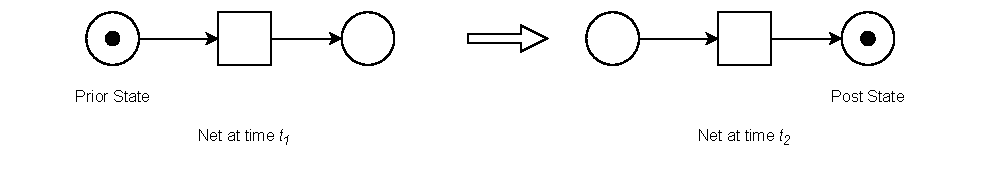
\includegraphics[width=\textwidth]{graphics/PN_Transduction.pdf}
\caption{\textbf{Transduction:
}The transducer is represented as a square node, which will fire when a condition of at least one token as input place value is satisfied, giving rise to the resulting place value.
Places are represented as circles with or without tokens (the values).}
\label{transduction}
\end{figure}

However, a pull action from the complement muscle between the cycle can generate a halting action in between.  Thus two actors can regulate each other's action without involving any other controlling agent or actor. A fine-grain halting may lead to greater coordination.  This is one model of implementing a simple haltable-action-pattern (HAP). 

Haltability, coordination of actions, emerges due to dynamic antagonism among the zones. Having established the fundamental principles of action and haltability, we now turn to the specific biological architecture that implements these principles. The SMN model proposes that cognition emerges from a particular body plan that is shared across animal life but has been largely ignored in cognitive science.

Antagonistic pairs realize physical implementations of reciprocal inhibition, giving SMN a robust substrate for $\mathcal{H}_\alpha$ (halt/phase-reset) without losing posture—key for safe interruptibility.

%=== Negotiable Action Patterns as conditional sequences ===
\paragraph{NAPs as conditional sequences.}
Negotiable Action Patterns (NAPs) can be thought of as \emph{action scripts} that unfold step by step, 
but with built-in checkpoints that test whether conditions are met. 
At each step, an action is performed while the environment is monitored; 
if the condition continues to hold, the action runs, but if it changes, the sequence can be halted, redirected, or switched to another action. 

In computer science, such conditional sequences are known as guarded traces \citep{Dijkstra1975,BaetenWeijland1990}: sequences of actions where each step executes only if its guard condition holds:  a sequence of actions ($a_1,a_2,\ldots,a_k$) paired with conditions ($g_1,g_2,\ldots,g_k$) that guard the transitions. Here we borrow the term not to stress its technical heritage but to capture the simple idea of actions unfolding under conditions, with the possibility of interruption or branching.

The haltability operator $\mathcal{H}_\alpha$ ensures that interruptions are safe: the agent can pause or reconfigure without collapsing its posture or coordination.

%--- Formal sketch (kept minimal) ---
\[
\gamma \;=\; (a_1, g_1)\to (a_2, g_2)\to \cdots \to (a_k, g_k), 
\qquad a_i\in \mathcal{A},\; g_i:\Sigma\to\{\top,\bot\}
\]

%--- Simple diagram ---
\begin{center}
\begin{tikzpicture}[node distance=16mm,>=stealth,auto,scale=0.95, every node/.style={transform shape}]
\node[draw,rounded corners,align=center,inner sep=3pt] (a1) {$a_1$\\(HAP/NAP)};
\node[draw,rounded corners,align=center,inner sep=3pt,right=of a1] (a2) {$a_2$};
\node[draw,rounded corners,align=center,inner sep=3pt,right=of a2] (a3) {$a_3$};
\path[->] (a1) edge node {$g_1$} (a2)
          (a2) edge node {$g_2$} (a3);
\path[->,dashed] (a2) edge[bend left=45] node[above] {$\mathcal{H}_{\alpha}$} (a1);
\path[->,dashed] (a2) edge[bend left=20] node[below] {$\mathcal{H}_{\beta}$} (a3);
\end{tikzpicture}
\end{center}
\vspace{-1ex}

In plain terms, a NAP is like a flexible habit or skill: it has a familiar structure, but the checkpoints (guards) and haltability make it negotiable and adaptable. 
When such NAPs leave traces that others can perceive—through gesture, voice, or external marks—they become \emph{Transactional Action Patterns} (TAPs), which enter the intersubjective domain of conversation and shared meaning \citep{Gibson1979,PezzuloCisek2016}.


%=== Negotiable Action Patterns as guarded traces ===
\paragraph{NAPs as guarded traces.}
Let $\mathcal{A}$ be the set of available HAP/NAP controllers and $\Sigma$ the set of perceptual predicates (affordance tests). 
A NAP can be expressed as a finite guarded trace
\[
\gamma \;=\; (a_1, g_1)\to (a_2, g_2)\to \cdots \to (a_k, g_k), 
\qquad a_i\in \mathcal{A},\; g_i:\Sigma\to\{\top,\bot\},
\]
executed by the policy
\[
\pi_\gamma(x) \;=\; 
\begin{cases}
\mathcal{H}_{\alpha_i}\!\circ a_i(x), & \text{while } g_i(\Sigma)=\top \\[4pt]
\text{branch to } (a_{i+1},g_{i+1}), & \text{on guard switch}.
\end{cases}
\]
Here $\mathcal{H}_{\alpha_i}$ denotes the haltability relation: it manages mid-course interruptions (pause, rephase, or re-route) without collapsing the pattern. 
This formalism captures how the SMN organizes flexible, negotiable action structures in an individual agent.

This schematizes NAPs as \emph{guarded compositions} of interruptible primitives. 
When such negotiable patterns are externalized into perceptible traces—gestural, vocal, or material—they become \emph{Transactional Action Patterns} (TAPs), entering the intersubjective domain where agents coordinate and converse \citep{Gibson1979,PezzuloCisek2016}.

\paragraph{Perceptual predicates (affordance tests).}
In the formal sketch of NAPs, each transition is guarded by a condition $g_i$. 
We call these conditions \emph{perceptual predicates} or \emph{affordance tests}. 
They are not abstract symbols but concrete checks the organism performs on its environment. 
Examples include:
\begin{itemize}
  \item \textbf{Motor–muscle level:} proprioceptors in flexor and extensor muscles signal whether the current joint angle or tension is within safe range; if a threshold is crossed, the ongoing action halts or adjusts. 
  \item \textbf{Sensorimotor level:} tactile receptors in the fingertips detect slippage during a grasp; this predicate triggers a branch from “lift” to “tighten grip.” 
  \item \textbf{Perceptual–ecological level:} vision and balance systems check whether a surface is flat and wide enough to step on; if not, the stepping routine is inhibited. 
  \item \textbf{Cognitive–social level:} auditory cues from a conversational partner signal that a turn has ended; the speaking action pattern is released in response.
\end{itemize}
Each of these can be written in the formalism as a binary test ($g_i:\Sigma \to \{\top,\bot\}$), but their richness lies in being embodied affordance checks, grounded in specific sensory modalities. 
They are the \emph{gates} that make NAPs negotiable: deciding whether to continue, halt, or branch without requiring abstract symbolic representation. 
Thus, perceptual predicates operationalize Gibson’s idea of affordances \citep{Gibson1979}, anchoring them in the agent’s bodily architecture and neural physiology.

\paragraph{Petri Nets as process models of SMN.}
While the idea of guarded traces has its origin in process algebra \citep{Dijkstra1975,BaetenWeijland1990}, 
for our purposes a more accessible and biologically faithful formalism is provided by \emph{Petri Nets} (PNs). 
PNs are bipartite graphs consisting of \emph{places} and \emph{transitions}, with directed arcs between them. 
In the SMN interpretation, the distributed processing units (DPUs)—flexor/extensor or left/right zones—are modeled as \emph{transitions}, 
while the mediated states carried by the central nervous system are modeled as \emph{places}. 
Tokens circulating through the net represent proprioceptive and sensory messages, with haltability implemented as gating conditions on token flow. 
This mapping makes visible how coordination emerges: when one zone is active (a transition firing), its partner zone is in an alert state, awaiting tokens for activation. 
Because Petri Nets have both a rigorous process algebra semantics and an intuitive graphical representation, they serve as an ideal bridge between formal dynamical models and multi-disciplinary accessibility.



% ==== PREAMBLE (if not already included) ====
% \usepackage{tikz}
% \usetikzlibrary{arrows.meta, positioning}
% \usepackage{tikzsymbols} % optional if you want token styles

% ==== PETRI NET DIAGRAM ====
\begin{figure}[t]
\centering
\begin{tikzpicture}[node distance=20mm,>=Stealth, every node/.style={transform shape}]
  % Places
  \node[place,tokens=1] (p1) {};
  \node[place,right=50mm of p1] (p2) {};

  % Transitions
  \node[transition,below=15mm of p1] (t1) {};
  \node[transition,below=15mm of p2] (t2) {};

  % Arcs
  \draw[->] (p1) -- (t1);
  \draw[->] (t1) -- (p2);
  \draw[->] (p2) -- (t2);
  \draw[->] (t2) -- (p1);
\end{tikzpicture}

\caption{Petri Net representation of a flexor--extensor antagonistic pair. 
Circles are \emph{places} (mediated CNS states carrying sensory tokens); 
rectangles are \emph{transitions} (local action zones/DPUs). 
Tokens (black dots) represent proprioceptive and sensory signals flowing through the system. 
Haltability corresponds to gating of token flow, ensuring that when one zone is active the antagonistic partner is in an alert state.}
\label{fig:pn-flexor-extensor}
\end{figure}

% ==== MULTI-ZONE SMN PETRI NET ====
\begin{figure}[t]
\centering
\begin{tikzpicture}[
  node distance=14mm and 20mm,
  >=Stealth,
  every node/.style={transform shape},
  tokenstyle/.style={place,minimum size=6mm},
  trstyle/.style={transition,minimum width=3mm,minimum height=10mm}
]

% ---------- Central broadcast place (CNS integration) ----------
\node[tokenstyle,tokens=2,label=above:{\footnotesize CNS broadcast state}] (CNS) {};

% ---------- ZONE A: Shoulder (Flexor/Extensor) ----------
% local proprioceptive place
\node[tokenstyle,tokens=1, left=36mm of CNS, yshift=18mm] (Aprop) {};
% transitions
\node[trstyle, below=10mm of Aprop,label=left:{\scriptsize A\_F}] (AF) {};
\node[trstyle, right=10mm of AF,label=right:{\scriptsize A\_E}] (AE) {};
% arcs (local)
\draw[->] (Aprop) -- (AF);
\draw[->] (Aprop) -- (AE);
% antagonistic loop via CNS
\draw[->] (AF) -- (CNS);
\draw[->] (AE) -- (CNS);

% ---------- ZONE B: Elbow ----------
\node[tokenstyle,tokens=1, left=36mm of CNS, yshift=-22mm] (Bprop) {};
\node[trstyle, below=10mm of Bprop,label=left:{\scriptsize B\_F}] (BF) {};
\node[trstyle, right=10mm of BF,label=right:{\scriptsize B\_E}] (BE) {};
\draw[->] (Bprop) -- (BF);
\draw[->] (Bprop) -- (BE);
\draw[->] (BF) -- (CNS);
\draw[->] (BE) -- (CNS);

% ---------- ZONE C: Wrist ----------
\node[tokenstyle,tokens=1, below=24mm of CNS, xshift=-10mm] (Cprop) {};
\node[trstyle, below=10mm of Cprop,label=left:{\scriptsize C\_F}] (CF) {};
\node[trstyle, right=10mm of CF,label=right:{\scriptsize C\_E}] (CE) {};
\draw[->] (Cprop) -- (CF);
\draw[->] (Cprop) -- (CE);
\draw[->] (CF) -- (CNS);
\draw[->] (CE) -- (CNS);

% ---------- ZONE D: Jaw ----------
\node[tokenstyle,tokens=1, right=36mm of CNS, yshift=12mm] (Dprop) {};
\node[trstyle, below=10mm of Dprop,label=left:{\scriptsize D\_F}] (DF) {};
\node[trstyle, right=10mm of DF,label=right:{\scriptsize D\_E}] (DE) {};
\draw[->] (Dprop) -- (DF);
\draw[->] (Dprop) -- (DE);
\draw[->] (DF) -- (CNS);
\draw[->] (DE) -- (CNS);

% ---------- ZONE E: Ankle ----------
\node[tokenstyle,tokens=1, right=36mm of CNS, yshift=-24mm] (Eprop) {};
\node[trstyle, below=10mm of Eprop,label=left:{\scriptsize E\_F}] (EF) {};
\node[trstyle, right=10mm of EF,label=right:{\scriptsize E\_E}] (EE) {};
\draw[->] (Eprop) -- (EF);
\draw[->] (Eprop) -- (EE);
\draw[->] (EF) -- (CNS);
\draw[->] (EE) -- (CNS);

% ---------- CNS-to-zone routing (examples) ----------
% (These show delivered/alert messages; keep sparse for clarity)
\draw[->, dashed] (CNS) to[bend left=20] (AF);
\draw[->, dashed] (CNS) to[bend left=12] (BE);
\draw[->, dashed] (CNS) to[bend right=15] (CE);
\draw[->, dashed] (CNS) to[bend right=18] (DF);
\draw[->, dashed] (CNS) to[bend right=10] (EE);

% ---------- Legend ----------
\node[anchor=north, align=left, below=50mm of CNS] (legend) {%
\begin{tabular}{@{}ll@{}}
\raisebox{1pt}{\tikz{\node[tokenstyle]{};}} & Place (state); dots = tokens (signals)\\
\raisebox{-1pt}{\tikz{\node[trstyle]{};}} & Transition (action zone DPU)\\
\raisebox{-1pt}{\tikz{\draw[->] (0,0) -- (0.8,0);}} & Routed token flow (firing/output)\\
\raisebox{-1pt}{\tikz{\draw[->,dashed] (0,0) -- (0.8,0);}} & Delivered/alert messages (haltability gates)\\
\end{tabular}
};

\end{tikzpicture}

\caption{Multi-zone Petri Net view of the SMN. Each antagonistic zone is modeled as a pair of \emph{transitions} (Flexor/Extensor DPUs) with a local proprioceptive \emph{place}. All zones write to a shared \emph{CNS broadcast place}, which routes messages and maintains an integrated body state. Solid arrows show token flow; dashed arrows depict routed “alert/haltability” deliveries.}
\label{fig:smn-multizone-pn}
\end{figure}

Tokens are proprioceptive/sensory messages; transitions fire when enabled by local tokens and CNS routing; dashed edges visualize haltability/alert delivery (readiness, not binary off). The shared CNS place implements broadcast/integration without central command.